\chapter{تداخل موجتين}\label{ch:b2:two-wave-interference}

فقاعة الصابون مصنوعة من سائل عديم اللون، ومع ذلك تتلألأ
بالألوان؛ وطبقة الزيت على طريق مبلّل تُظهر أشرطة قوس القزح نفسها؛
وجناحا اليعسوب يلمعان أخضر وبنفسجيًّا. وليس شيء من هذه الألوان
آتيًا من صباغ: بل من نسختين من موجة الضوء نفسها،
تنعكسان على وجهي غشاء رقيق، وتصلان بتأخير
فتتعاضدان أو تتلاشيان --- وهو \emph{تداخل}
موجتين. وقد جعله يونغ عام 1801 برهانًا على أن الضوء موجة،
بشقّين وشمعة؛ وهذا الفصل يعرض الصيغة، وهندسة
هدب يونغ، والشرطين --- الترابط الزماني \omterm{prop:b2:two-wave-interference:spatial}{والترابط
المكاني} --- اللذين تبقى الهدب بهما، وألوان الأغشية
الرقيقة.

\begin{omfigure}
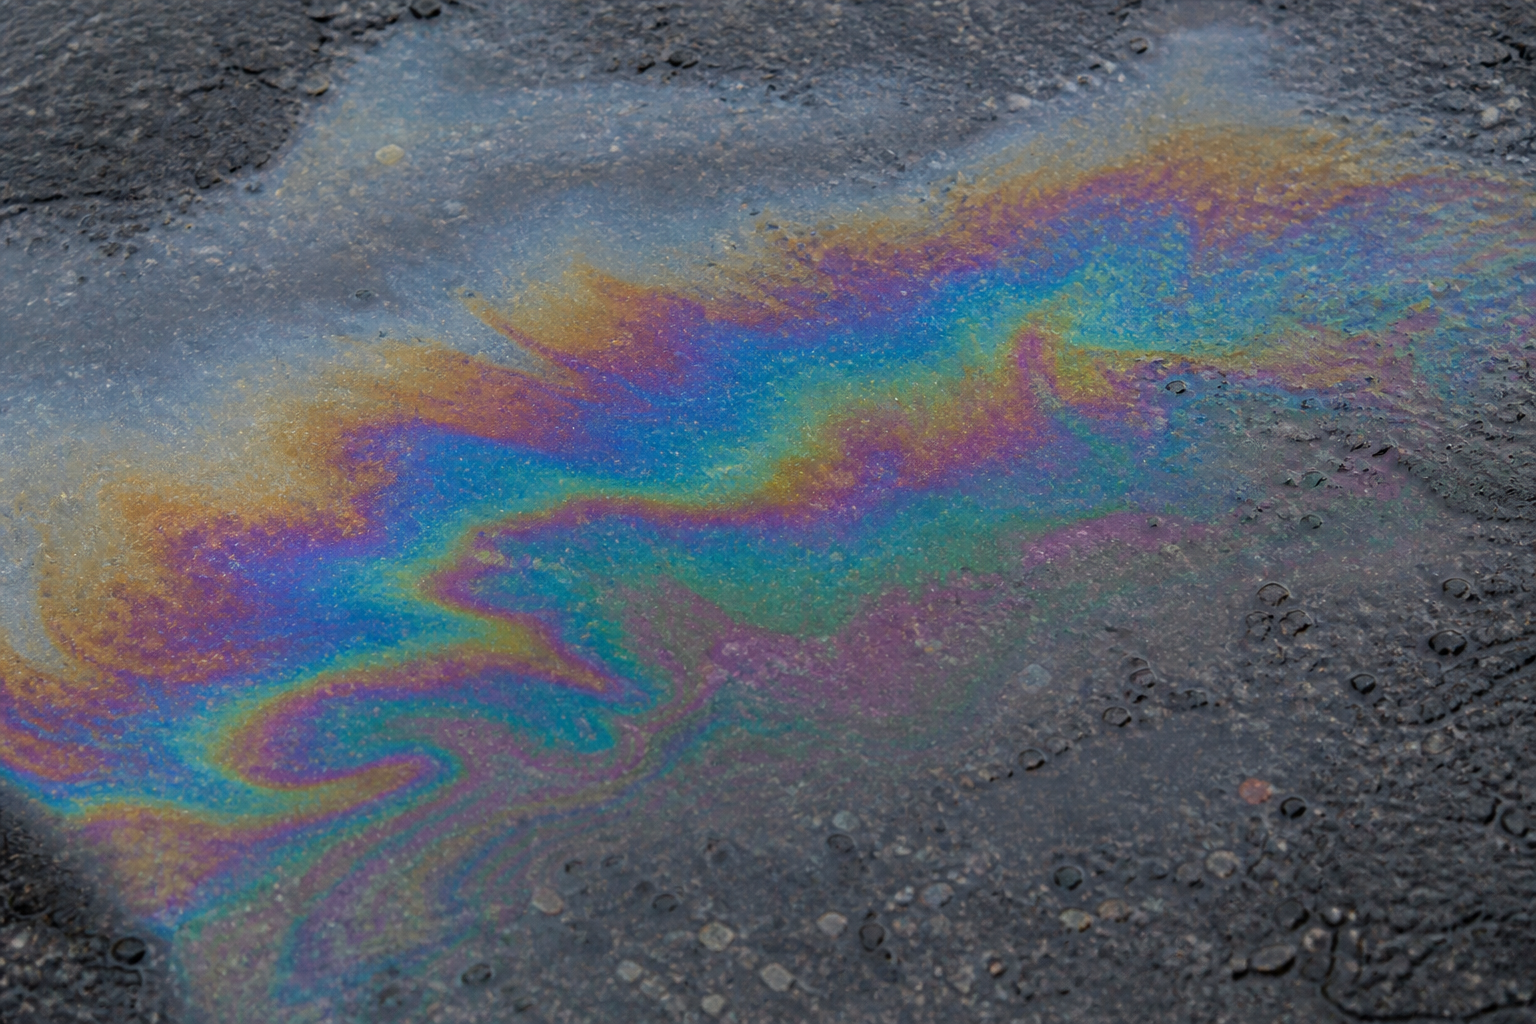
\includegraphics[width=0.58\linewidth]{images/book4/ai/b4-19-oil-film-puddle.png}

{\small غشاء زيت على طريق مبلّل: انعكاسان، واحد من كل وجه، وسماكة تتغير من موضع إلى آخر --- فكل لون مضيء حيث تكون للمقدار $2ne$ القيمة الصحيحة.}
\end{omfigure}


\section{صيغة التداخل}

\begin{theorem}[تداخل موجتين]\label{thm:b2:two-wave-interference:formula}
\index{تداخل}\index{فرق المسير}\index{رتبة التداخل}\index{تباين (الهدب)}
موجتان مترابطتان أحاديتا اللون شدتاهما $I_1$ و $I_2$ وفرق طورهما
$\Delta\varphi$ عند نقطة $M$ تعطيان هناك الشدة
\[
I(M) = I_1 + I_2 + 2\sqrt{I_1I_2}\,\cos\Delta\varphi(M) , \qquad
\Delta\varphi = \frac{2\pi}{\lambda_0}\,\delta(M) ,
\]
حيث $\delta$ هو \emph{\omterm{thm:b2:two-wave-interference:formula}{فرق المسير} الضوئي} بين
الطريقين من المنبع إلى $M$. والشدة عظمى ($I_1 + I_2 +
2\sqrt{I_1I_2}$) حيث $\delta = p\lambda_0$، و $p$ عدد صحيح --- وهو \emph{\omterm{thm:b2:two-wave-interference:formula}{رتبة
التداخل}} --- وصغرى ($I_1 + I_2 - 2\sqrt{I_1I_2}$) حيث $\delta = (p +
\tfrac12)\lambda_0$. و\emph{تباين} الهدب (أي وضوحها) هو
\[
V = \frac{I_{\max} - I_{\min}}{I_{\max} + I_{\min}} = \frac{2\sqrt{I_1I_2}}{I_1 + I_2} ,
\]
وهو يساوي $1$ من أجل شدتين متساويتين، حيث تكون مواضع الصغر مظلمة تمامًا:
$I = 2I_0(1 + \cos\Delta\varphi) = 4I_0\cos^2(\Delta\varphi/2)$.
\end{theorem}

\begin{proof}
$s = a_1\cos(\omega t - \varphi_1) + a_2\cos(\omega t - \varphi_2)$؛ و $\langle s^2\rangle$ كما في
\cref{ch:b2:scalar-light-model}، مع $\Delta\varphi$ ثابتًا في أثناء
الكشف؛ و $I_i = \tfrac12Ka_i^2$. وفرق طور موجتين
غادرتا المنبع معًا وقطعتا المسيرين الضوئيين $L_1$ و $L_2$ هو
$2\pi(L_2 - L_1)/\lambda_0$ (زائدًا $\pi$ عن كل انعكاس يعكس
الإشارة، \cref{ch:b2:wave-interfaces}).
\end{proof}

\begin{remark}[الشروط الثلاثة]\label{rem:b2:two-wave-interference:conditions}
\index{ترابط (مكاني)}\index{ترابط (زماني)}
لا توجد الهدب إلا إذا (1) جاءت الموجتان من \emph{المنبع
نفسه} (أي نسختين من اهتزاز واحد، وإلا كان $\Delta\varphi$ عشوائيًّا)؛ (2)
وكان \omterm{thm:b2:two-wave-interference:formula}{فرق المسير} أصغر من \omterm{prop:b2:scalar-light-model:coherence}{طول الترابط}، $|\delta| < \ell_c$
(وهو \emph{الترابط الزماني}: إذ تنتمي النسختان وراءه إلى قطارين
موجيين مختلفين)؛ (3) وكان المنبع صغيرًا كفاية بحيث لا تعطي نقاطه
المختلفة نظم هدب متزاحة يمحو بعضها بعضًا
(وهو \emph{\omterm{prop:b2:two-wave-interference:spatial}{الترابط المكاني}}، أدناه). ورابع، وهو متحقق عادةً:
ألا يكون للموجتين استقطابان متعامدان (إذ تتجمعان
عندئذ في الشدة، كالمصباحين اليدويين).
\end{remark}

\section{شقّا يونغ}

\begin{proposition}[تقسيم جبهة الموجة: تجربة يونغ]\label{prop:b2:two-wave-interference:young}
\index{شقّا يونغ}\index{البعد الهدبي}\index{تقسيم جبهة الموجة}
منبع نقطي $S$ (أو شقّ) يضيء شقّين ضيّقين متوازيين
$S_1$ و $S_2$ يتباعدان $a$، ويبعدان عن $S$ بالسواء؛ وتقوم شاشة على
البعد $D \gg a$. وعند نقطة الشاشة الواقعة على الارتفاع $x$ (الموازي
\omterm{def:b2:maxwell-equations:operators}{للتباعد} $a$) يكون \omterm{thm:b2:two-wave-interference:formula}{فرق المسير}
\[
\delta = S_2M - S_1M \approx \frac{ax}D ,
\]
وتُظهر الشاشة هدبًا مستقيمة متساوية \omterm{def:b2:maxwell-equations:operators}{التباعد}، مضيئةً عند $x_p =
p\lambda D/a$، و\emph{\omterm{prop:b2:two-wave-interference:young}{البعد الهدبي}} هو
\[
i = \frac{\lambda D}a .
\]
وتوجد الهدب في كل مكان خلف الشقّين (فهي \emph{غير
موضَّعة})؛ ومع عدسة بعدها البؤري $f$ بعد الشقّين، تُرى
في مستويها البؤري \omterm{prop:b2:two-wave-interference:young}{بالبعد الهدبي} $i = \lambda f/a$ (أي هدب "في اللانهاية").
والشدة هي $4I_0\cos^2(\pi ax/\lambda D)$.
\end{proposition}

\begin{proof}
$S_2M^2 - S_1M^2 = [(x + a/2)^2 - (x - a/2)^2] = 2ax$ و $S_2M + S_1M \approx 2D$،
ومن ثَمّ $\delta \approx 2ax/2D$. ورتبتان متتاليتان تختلفان بمقدار $\lambda$، أي بمقدار $\Delta x = \lambda D/a$.
ومع عدسة يكون للموجتين الخارجتين من الشقّين تحت الزاوية $\theta$ عن
المحور \omterm{thm:b2:two-wave-interference:formula}{فرق المسير} $a\sin\theta \approx a\theta$ وتلتقيان عند $x = f\theta$.
\end{proof}

\begin{omfigure}
\begin{tikzpicture}[font=\small, x=1cm, y=1cm, >=Stealth]
  \begin{scope}
    \fill (-3.6,0) circle (1.5pt); \node[font=\footnotesize] at (-3.8,0.3) {$S$};
    \draw[thick] (-1.5,-1.6) -- (-1.5,-0.35) (-1.5,-0.15) -- (-1.5,0.15) (-1.5,0.35) -- (-1.5,1.6);
    \fill (-1.5,0.25) circle (1.2pt) node[left, font=\footnotesize] {$S_1$}; \fill (-1.5,-0.25) circle (1.2pt) node[left, font=\footnotesize] {$S_2$};
    \draw[<->] (-1.1,0.25) -- (-1.1,-0.25) node[midway, right, font=\footnotesize] {$a$};
    \draw[thick] (2.8,-1.8) -- (2.8,1.8);
    \fill (2.8,0.9) circle (1.5pt) node[right, font=\footnotesize] {$M$, $x$};
    \draw[omDef, thick] (-1.5,0.25) -- (2.8,0.9); \draw[omDef, thick] (-1.5,-0.25) -- (2.8,0.9);
    \draw[omDef, thick] (-3.6,0) -- (-1.5,0.25); \draw[omDef, thick] (-3.6,0) -- (-1.5,-0.25);
    \draw[<->] (-1.5,-2.0) -- (2.8,-2.0) node[midway, below, font=\footnotesize] {$D$};
    \node[font=\footnotesize] at (0.6,-1.5) {$\delta \approx ax/D$};
    % الهدب على الشاشة
    \foreach \y in {-1.5,-1.0,-0.5,0,0.5,1.0,1.5} \fill[omThm!50] (2.85,{\y-0.12}) rectangle (3.15,{\y+0.12});
    \draw[<->] (3.35,0) -- (3.35,0.5) node[midway, right, font=\footnotesize] {$i$};
  \end{scope}
  \begin{scope}[xshift=9.3cm]
    \begin{axis}[omaxis, axis x line=bottom, axis y line=left, width=4.2cm, height=4.0cm, at={(0,-1.7cm)},
        xlabel={$x/i$}, ylabel={$I/I_0$}, xmin=-2.5, xmax=2.5, ymin=0, ymax=4.4, xtick={-2,-1,0,1,2}, ytick={2,4}, samples=200,
        xlabel style={at={(axis description cs:0.5,-0.14)}, anchor=north},
        ylabel style={at={(axis description cs:-0.12,0.5)}, rotate=90, anchor=south}]
      \addplot[omDef, thick, domain=-2.5:2.5] {4*cos(deg(pi*x))^2};
      \addplot[omThm, thick, dashed, domain=-2.5:2.5] {2+1.2*cos(deg(2*pi*x))};
    \end{axis}
  \end{scope}
\end{tikzpicture}

{\small على اليسار: \omterm{prop:b2:two-wave-interference:young}{شقّا يونغ} --- نسختان من موجة المنبع تلتقيان على
الشاشة \omterm{thm:b2:two-wave-interference:formula}{بفرق المسير} $ax/D$؛ وهدبة مضيئة كل
$\lambda D/a$. وعلى اليمين: مقطع الشدة، $4I_0\cos^2(\pi x/i)$ من أجل موجتين
متساويتين (بخط متصل) ومع تباين منخفض (بخط متقطع).}
\end{omfigure}

\begin{example}[أرقام، وضوء أبيض]\label{ex:b2:two-wave-interference:numbers}
$a = \qty{0.5}{mm}$، و $D = \qty{2}{m}$، و $\lambda = \qty{600}{nm}$: $i = \qty{2.4}{mm}$ --- أي كبير
كفاية ليُرى، ولهذا وجب أن يتقارب \omterm{prop:b2:two-wave-interference:young}{شقّا يونغ} وتبعد
الشاشة. وفي الضوء الأبيض يصنع كل لون هدبه، وكلها
تتطابق في المركز ($\delta = 0$): فهدبة مركزية بيضاء، ثم
هدب ملونة كلما تباعدت الرتب ($i$ الأحمر $1.8$ ضعف
البنفسجي)، وبعد بضع رتب حقل أبيض منتظم --- إذ
طول ترابط الضوء الأبيض ميكرومتر، أي طولا موجة أو ثلاثة.
والمطياف الموجَّه إلى ذلك الحقل "الأبيض" يرى مع ذلك
أشرطة مظلمة عند أطوال الموجة التي من أجلها $\delta = (p + \tfrac12)\lambda$: وهو
\emph{طيف مخدَّد}.
\end{example}

\begin{proposition}[الترابط المكاني: يجب أن يكون المنبع صغيرًا]\label{prop:b2:two-wave-interference:spatial}
\index{ترابط مكاني}\index{منبع ممتد}
كل نقطة من \omterm{prop:b2:two-wave-interference:spatial}{منبع ممتد} تعطي نظام هدبها؛ ونقطة
منبع مزاحة مستعرضًا بمقدار $b$ على البعد $L$ قبل
الشقّين تزيح الهدب بمقدار $x = bD/L$ (إذ يكسب \omterm{thm:b2:two-wave-interference:formula}{فرق المسير}
$ab/L$). ومنبع عرضه $b$ ينشر الهدب على بعد هدبي واحد،
فيزول التباين، حين يكون
\[
\frac{ab}L \approx \lambda , \qquad\text{أي حين يرى الشقّان المنبع تحت زاوية } \frac bL \gtrsim \frac\lambda a .
\]
ويجب أن يقع الشقّان داخل \emph{مساحة ترابط} الضوء ---
أي المنطقة التي يكون فيها للموجة الآتية من المنبع طور معيّن،
وعرضها $\lambda L/b$. وضوء الشمس ($b/L = \qty{0.5}{\degree} = \qty{9}{mrad}$)
يعطي عرض ترابط $\lambda/0.009 \approx \qty{60}{\micro m}$: ولذلك احتاج يونغ إلى
ثقب دبوس ليوسّعه.
\end{proposition}

\begin{proof}
من أجل نقطة منبع على الارتفاع $b$، يضاف المسير الزائد $SS_2 - SS_1 \approx -ab/L$
إلى $ax/D$: فينزاح النقش بمقدار $x = bD/L$. ومكاملة نقوش
$\cos^2$ المزاحة على منبع عرضه $b$ تعطي تباينًا
$|\operatorname{sinc}(\pi ab/\lambda L)|$، وهو معدوم عند $ab/L = \lambda$.
\end{proof}

\begin{omfigure}
\begin{tikzpicture}[font=\small, x=1cm, y=1cm, >=Stealth]
  \draw[thick, omThm] (-4.2,-0.4) -- (-4.2,0.4); \node[omThm, font=\footnotesize] at (-4.6,0) {$b$};
  \draw[thick] (-1.0,-1.5) -- (-1.0,-0.3) (-1.0,-0.1) -- (-1.0,0.1) (-1.0,0.3) -- (-1.0,1.5);
  \draw[omDef] (-4.2,0.4) -- (-1.0,0.2); \draw[omDef] (-4.2,0.4) -- (-1.0,-0.2);
  \draw[omProp] (-4.2,-0.4) -- (-1.0,0.2); \draw[omProp] (-4.2,-0.4) -- (-1.0,-0.2);
  \draw[<->] (-4.2,-1.9) -- (-1.0,-1.9) node[midway, below, font=\footnotesize] {$L$};
  \draw[thick] (3.0,-1.8) -- (3.0,1.8);
  \foreach \y in {-1.5,-1.0,-0.5,0,0.5,1.0,1.5} \fill[omDef!50] (3.05,{\y-0.1}) rectangle (3.3,{\y+0.1});
  \foreach \y in {-1.5,-1.0,-0.5,0,0.5,1.0,1.5} \fill[omProp!50] (3.35,{\y-0.1+0.25}) rectangle (3.6,{\y+0.1+0.25});
  \node[font=\footnotesize] at (-0.5,2.2) {كل نقطة منبع: هدبها هي، مزاحة بمقدار $bD/L$};
  \node[font=\footnotesize] at (-0.5,-2.5) {يضيع التباين حين $ab/L \approx \lambda$};
\end{tikzpicture}

{\small \omterm{prop:b2:two-wave-interference:spatial}{الترابط المكاني}: أعلى \omterm{prop:b2:two-wave-interference:spatial}{المنبع الممتد} وأسفله
يرسلان نظامي هدب مزاحًا أحدهما عن الآخر؛ وحين تبلغ الإزاحة
بعدًا هدبيًّا واحدًا يُمحى النقش.}
\end{omfigure}

\section{الأغشية الرقيقة: تقسيم السعة}

\begin{proposition}[التداخل في غشاء رقيق]\label{prop:b2:two-wave-interference:film}
\index{تداخل الأغشية الرقيقة}\index{تقسيم السعة}\index{هدب تساوي الميل}\index{هدب تساوي السماكة}
غشاء قرينته $n$ وسماكته $e$ في الهواء، مضاء تحت الورود $i$
(وزاوية الانكسار $r$)، يعيد موجتين تنعكسان على وجهيه،
\omterm{thm:b2:two-wave-interference:formula}{بفرق المسير}
\[
\delta = 2ne\cos r \ (+\tfrac{\lambda_0}2) ,
\]
حيث يعدّ نصف طول الموجة الزائد انعكاسَ الإشارة عند الانعكاس
على الوسط الأكثف عند الوجه الأول لا عند الثاني
(\cref{ch:b2:wave-interfaces}). والهدب مضيئة عند $2ne\cos r =
(p + \tfrac12)\lambda_0$، ومظلمة عند $2ne\cos r = p\lambda_0$ --- والغشاء المتلاشي
السماكة لا يعكس \emph{شيئًا} (وهو أعلى غشاء الصابون الأسود
حين ينزف). وفي غشاء منتظم السماكة تتعلق الهدب بالورود $i$ وحده
وتُرى في اللانهاية (حلقات \emph{تساوي الميل})؛ وفي إسفين
بطيء تغير السماكة يُنظر إليه قرب الورود الناظمي تتبع الهدب
خطوط تساوي $e$ وتُوضَّع على الغشاء
(هدب \emph{تساوي السماكة}): فإسفين هوائي زاويته $\alpha$ يُظهر
هدبًا مستقيمة متباعدة $\lambda_0/2\alpha$؛ وعدسة نصف قطرها $R$ على مستوٍ تعطي
\emph{حلقات نيوتن}، مظلمة عند $r_p = \sqrt{p\lambda_0R}$.
\end{proposition}

\begin{proof}
أما الهندسة: فالموجة المنكسرة عند الوجه الأول تعبر الغشاء مرتين
($2e/\cos r$ في الزجاج، \omterm{def:b2:scalar-light-model:path}{والمسير الضوئي} $2ne/\cos r$) بينما تتقدم الموجة المنعكسة
عند الوجه الأول $2e\tan r\sin i$ في الهواء؛ والفرق هو
$2ne/\cos r - 2e\tan r\sin i = 2ne\cos r$ مع $\sin i = n\sin r$. وأما
الإسفين: فيكون $e = \alpha x$ والهدب المظلمة المتتالية عند $2\alpha x = p\lambda$؛ وأما العدسة:
فيكون $e \approx r^2/2R$.
\end{proof}

\begin{omfigure}
\begin{tikzpicture}[font=\small, x=1cm, y=1cm, >=Stealth]
  \begin{scope}
    \fill[omDef!15] (-3,-0.9) rectangle (3,0.9); \draw[thick] (-3,0.9) -- (3,0.9) (-3,-0.9) -- (3,-0.9);
    \node[font=\footnotesize] at (2.4,0) {$n$}; \draw[<->] (-2.7,-0.9) -- (-2.7,0.9) node[midway, left, font=\footnotesize] {$e$};
    \draw[omThm, thick, ->] (-2.2,2.2) -- (-0.9,0.95);
    \draw[omThm, thick, ->] (-0.85,0.92) -- (0.4,2.2);
    \draw[omProp, thick] (-0.9,0.9) -- (-0.2,-0.9) -- (0.5,0.9);
    \draw[omProp, thick, ->] (0.5,0.92) -- (1.75,2.2);
    \node[font=\footnotesize] at (-1.7,1.85) {$i$}; \node[font=\footnotesize] at (-0.75,-0.0) {$r$};
    \node[font=\footnotesize] at (0,-1.4) {$\delta = 2ne\cos r$ (+ $\lambda/2$)};
  \end{scope}
  \begin{scope}[xshift=7.8cm]
    \draw[thick] (-2.6,0) -- (2.6,0);
    \draw[thick] (-2.6,0.05) arc[start angle=-90, end angle=-60, radius=14] ;
    \draw[thick] (-2.6,0.05) -- (2.6,0.55);
    \foreach \x in {-2.0,-1.3,-0.6,0.1,0.8,1.5,2.2} \draw[omThm, very thick] (\x,-0.25) -- (\x,-0.45);
    \node[font=\footnotesize] at (0,-0.85) {إسفين هوائي: هدبة مظلمة كل $\lambda/2\alpha$};
    \draw[omDef, thick] (-2.6,0.05) -- (-2.6,0); \node[font=\footnotesize] at (2.9,0.3) {$\alpha$};
  \end{scope}
\end{tikzpicture}

{\small على اليسار: الانعكاسان من غشاء رقيق --- واحد من كل
وجه، والثاني متأخر بالعبور المضاعف. وعلى اليمين: إسفين هوائي
بين صفيحتين يُظهر هدبًا مستقيمة متساوية السماكة، واحدة في كل
نصف طول موجة من الفرجة الزائدة.}
\end{omfigure}

\begin{example}[الصابون والزيت واليعاسيب]\label{ex:b2:two-wave-interference:colours}
غشاء صابون ($n = 1.33$) سماكته \qty{300}{nm} يُنظر إليه على الورود الناظمي:
يكون مضيئًا عند $2ne = (p + \tfrac12)\lambda$، أي $\lambda = 798/(p + \tfrac12)$ نانومتر: \qty{532}{nm}
(أخضر، $p = 1$) ضمن المرئي، مع شريط مظلم عند \qty{400}{nm}؛
فيبدو الغشاء أخضر. وكلما نزف ورقّ جرى اللون في
التتابع، منتهيًا إلى السواد. وأما غشاء زيت (\qty{400}{nm}، $n = 1.45$) على ماء
($1.33$): فالانعكاس الثاني، نحو قرينة أدنى، لا يعكس
الإشارة، فيكون $\delta = 2ne + \lambda/2$ أيضًا ويكون الغشاء مضيئًا عند $2ne =
(p + \tfrac12)\lambda$: \qty{464}{nm} ($p = 2$)، أي أزرق. وتلألؤ
جناح الفراشة، وصدفة الخنفساء، والقرص المدمج تداخلات
من النوع نفسه (وأما تداخل القرص فبأمواج كثيرة: \cref{ch:b2:gratings})،
ولذلك تتغير مع الزاوية --- إذ يتعلق $\delta$ بالمقدار $\cos r$ ---
بينما لا يتغير لون الصباغ.
\end{example}

\begin{method}[حلّ مسألة تداخل]\label{met:b2:two-wave-interference:method}
(1) عيّن الطريقين من المنبع إلى $M$ واحسب
\omterm{thm:b2:two-wave-interference:formula}{فرق المسير} الضوئي $\delta(M)$، مضيفًا $\lambda/2$ عن كل انعكاس
تنعكس فيه الإشارة. (2) و $I = I_1 + I_2 + 2\sqrt{I_1I_2}\cos(2\pi\delta/\lambda)$؛
وهي مضيئة عند $\delta = p\lambda$. (3) \omterm{def:b2:maxwell-equations:operators}{وتباعد} الهدب من $\delta(M + \Delta M) - \delta(M) =
\lambda$. (4) وتحقق من الترابط الزماني ($\delta_{\max} < \ell_c$، وعدد
الهدب المرئية $\sim\lambda/\Delta\lambda$) ومن \omterm{prop:b2:two-wave-interference:spatial}{الترابط المكاني} (زاوية المنبع
$< \lambda/a$). (5) وقل أين تُوضَّع الهدب (في كل مكان من أجل منبعين
نقطيين؛ وعلى الغشاء من أجل \omterm{prop:b2:two-wave-interference:film}{هدب تساوي السماكة}؛ وفي اللانهاية
من أجل \omterm{prop:b2:two-wave-interference:film}{هدب تساوي الميل}).
\end{method}

\section{تمارين}

\begin{exercise}[$\star$]\label{exo:b2:two-wave-interference:1}
\omterm{prop:b2:two-wave-interference:young}{شقّا يونغ} متباعدان $a = \qty{0.40}{mm}$، والشاشة على $D = \qty{1.5}{m}$، و $\lambda =
\qty{633}{nm}$: أوجد \omterm{prop:b2:two-wave-interference:young}{البعد الهدبي}؛ ورتبة الهدبة عند $x = \qty{1.0}{cm}$؛ وموضع
الهدبة المظلمة العاشرة؛ \omterm{prop:b2:two-wave-interference:young}{والبعد الهدبي} إذا \omterm{def:b2:maxwell-equations:operators}{تباعد} الشقّان \qty{2}{mm}،
وفي الماء ($n = 1.33$).
\end{exercise}

\begin{exercise}[$\star$]\label{exo:b2:two-wave-interference:2}
موجتان شدتاهما $I_0$ و $I_0/4$ تتداخلان: أوجد $I_{\max}$، و $I_{\min}$،
والتباين. وأعد ذلك من أجل $I_0$ و $I_0/100$: ولمَ تبقى الهدب مرئية
مع حزمتين بهذا التفاوت؟ ويُغطّى أحد شقّي يونغ بمرشّح
رمادي ينفذ $50\%$: أوجد التباين الجديد.
\end{exercise}

\begin{exercise}[$\star$]\label{exo:b2:two-wave-interference:3}
غشاء صابون سماكته \qty{250}{nm} ($n = 1.33$) يُنظر إليه على الورود الناظمي:
أوجد أطوال الموجة المرئية الأكثر انعكاسًا والأقلّ؛ ولونه. وغشاء
سماكته \qty{1.0}{\micro m}: كم طول موجة مضيئًا في المرئي، وماذا
ترى العين؟
\end{exercise}

\begin{exercise}[$\star$]\label{exo:b2:two-wave-interference:4}
حلقات نيوتن بين عدسة نصف قطرها $R = \qty{2.0}{m}$ ومستوٍ، في
ضوء الصوديوم: أوجد أنصاف أقطار أول ثلاث حلقات مظلمة؛ وعدد الحلقات
ضمن نصف قطر \qty{1}{cm}؛ أيكون المركز مضيئًا أم مظلمًا، ولماذا؟
وما الذي يتغير إذا مُلئت الفرجة بالماء؟
\end{exercise}

\begin{exercise}[$\star\star$]\label{exo:b2:two-wave-interference:5}
\emph{الضوء الأبيض.} \omterm{prop:b2:two-wave-interference:young}{شقّا يونغ} بضوء أبيض ($400$--\qty{700}{nm})،
و $a = \qty{0.5}{mm}$، و $D = \qty{1}{m}$. (أ) أوجد \omterm{prop:b2:two-wave-interference:young}{البعد الهدبي} للبنفسجي وللأحمر؛
وموضع الهدبتين المضيئتين الثانية الحمراء والثالثة البنفسجية. (ب)
وبعد أي رتبة تتراكب هدب الأحمر والبنفسجي من الرتب المتتالية؟
(ج) وعند $x = \qty{5}{mm}$، أي أطوال الموجة غائبة
(أي الطيف المخدَّد)؟ (د) وفسّر تتابع الألوان المرئي من
المركز نحو الخارج.
\end{exercise}

\begin{exercise}[$\star\star$]\label{exo:b2:two-wave-interference:6}
\emph{حجم المنبع.} مصباح صوديوم يضيء شقّي يونغ ($a = \qty{1.0}{mm}$)
عبر شقّ منبع على $L = \qty{40}{cm}$. (أ) أوجد أعظم عرض
لشقّ المنبع من أجل تباين جيد (خذ $ab/L < \lambda/4$). (ب) ويُوسَّع شقّ المنبع
إلى \qty{0.5}{mm}: أوجد التباين (باستعمال $|\operatorname{sinc}(\pi ab/\lambda L)|$).
(ج) ولمَ لا يمكن استعمال المصباح العاري (وعرضه \qty{1}{cm})؟ (د) والشمس
منبعًا، وعرضها \qty{9}{mrad}: أوجد أعظم \omterm{def:b2:maxwell-equations:operators}{تباعد} بين الشقّين يعطي
هدبًا.
\end{exercise}

\begin{exercise}[$\star\star$]\label{exo:b2:two-wave-interference:7}
\emph{مرآة لويد.} منبع نقطي على ارتفاع $h = \qty{0.2}{mm}$ فوق
مرآة مستوية، والشاشة على $D = \qty{1.0}{m}$، و $\lambda = \qty{500}{nm}$: تتداخل الموجة المباشرة
مع المنعكسة على المرآة (أي منبع تخيلي عند
$-h$). (أ) أوجد \omterm{prop:b2:two-wave-interference:young}{البعد الهدبي}. (ب) والهدبة عند حرف المرآة ($x = 0$)
مظلمة: فماذا يقول ذلك عن الانعكاس؟ (ج) وأوجد عدد الهدب
المرئية إذا كان طول ترابط المنبع \qty{50}{\micro m}. (د) ولمَ يكون
هذا الترتيب "مقياس تداخل البحر" عند الفلكي الراديوي من أجل نجم صاعد؟
\end{exercise}

\begin{exercise}[$\star\star$]\label{exo:b2:two-wave-interference:8}
\emph{الإسفين الهوائي.} صفيحتان زجاجيتان طولهما \qty{10}{cm} تتلامسان عند طرف
وتفصلهما عند الآخر شعرة قطرها $d$؛ وفي ضوء الصوديوم
تُعدّ $42$ هدبة مظلمة. (أ) أوجد $d$. (ب) \omterm{def:b2:maxwell-equations:operators}{وتباعد} الهدب. (ج) وتُملأ الفرجة
بالماء: أوجد عدد الهدب. (د) وتُضغط الصفيحتان قليلًا عند الطرف البعيد:
فماذا تفعل الهدب، وأي دقة على
$d$ يعطيها عدّ ربع هدبة؟
\end{exercise}

\begin{exercise}[$\star\star$]\label{exo:b2:two-wave-interference:9}
\emph{زيت على ماء.} غشاء زيت ($n = 1.45$) سماكته $e$ يطفو
على ماء ($n = 1.33$). (أ) أيّ الانعكاسين يعكس
الإشارة؟ وأوجد \omterm{thm:b2:two-wave-interference:formula}{فرق المسير}. (ب) ومن أجل $e = \qty{400}{nm}$ على الورود الناظمي:
أوجد أطوال الموجة المنعكسة المتعاضدة والمتلاشية؛ واللون. (ج) وأرقّ
غشاء يبدو بنفسجيًّا (\qty{420}{nm}). (د) ولمَ تنزاح الألوان نحو
الأزرق حين يُنظر إلى الغشاء مائلًا؟ (ه) وما الذي يتغير من أجل غشاء
تقع قرينته \emph{بين} قرينتي الوسطين (أي طلاء على
زجاج)؟
\end{exercise}

\begin{exercise}[$\star\star\star$]\label{exo:b2:two-wave-interference:10}
\emph{شريحة على أحد الشقّين.} صفيحة زجاجية سماكتها $e = \qty{20}{\micro m}$
وقرينتها $1.5$ تغطي الشقّ $S_1$ من زوج يونغ ($a = \qty{1}{mm}$، و $D =
\qty{2}{m}$، و $\lambda = \qty{500}{nm}$). (أ) أوجد \omterm{def:b2:scalar-light-model:path}{المسير الضوئي} الزائد؛ وبكم هدبة
وفي أي جهة ينزاح النقش؟ (ب) وفي الضوء الأبيض،
إلى أين تذهب الهدبة المركزية البيضاء (المزاحة الآن) --- أتبقى
مرئية؟ \omterm{prop:b2:scalar-light-model:coherence}{وطول الترابط} \qty{1.5}{\micro m}. (ج) واستعمل نقش الضوء الأبيض
لقياس $e$: كيف؟ (د) وتُمال الصفيحة: فتكبر الإزاحة
--- بيّن أنها تكبر من المرتبة الأولى وفق $e(n - 1)\theta^2/2 \times (1 + 1/n)$
وقدّرها من أجل \qty{5}{\degree}.
\end{exercise}

\begin{exercise}[$\star\star\star$]\label{exo:b2:two-wave-interference:11}
\emph{مقياس التداخل النجمي.} مرآتان متباعدتان $a$
تجمعان ضوء نجم وتجعلانه يتداخل. والنجم قرص
منتظم قطره الزاوي $\theta$؛ وكل نقطة منه تزيح
الهدب، ويزول التباين عند $a = 1.22\lambda/\theta$ (وهو مقبول، أي صيغة
القرص من $ab/L = \lambda$). (أ) ومن أجل منكب الجوزاء، $\theta = \qty{0.047}{''}$
(بالثواني القوسية)، و $\lambda = \qty{570}{nm}$: أوجد قاعدة القياس التي تختفي عندها
الهدب (ميكلسون، 1920، جبل ويلسون). (ب) ولمَ لا يستطيع مقراب
واحد قطره \qty{2.5}{m} أن يفصل القرص (وحدّه $1.22\lambda/d$)؟
(ج) وتربط مقاييس التداخل الحديثة مقاريب متباعدة \qty{100}{m}: أوجد أصغر
قطر يمكن قياسه. (د) ولمَ يجب أن يتساوى المسيران في حدود
\omterm{prop:b2:scalar-light-model:coherence}{طول الترابط}، وكم يبلغ ذلك من أجل مرشّح \qty{10}{nm}؟
\end{exercise}

\begin{exercise}[$\star\star\star$]\label{exo:b2:two-wave-interference:12}
\emph{حلقات تساوي الميل.} صفيحة متوازية الوجهين سماكتها $e =
\qty{2.0}{mm}$ وقرينتها $1.5$ يضيئها منبع صوديوم عريض؛ ويُجمَّع
الضوء المنعكس بعدسة $f = \qty{50}{cm}$. (أ) بيّن أن
الحلقات تقع عند الزوايا $i_p$ حيث $2ne\cos r_p = (p + \tfrac12)\lambda$ (مضيئة)
وأنه، قرب المركز، $\cos r \approx 1 - i^2/2n^2$. (ب) وأوجد الرتبة عند
المركز؛ أيكون المركز مضيئًا؟ (ج) وأنصاف أقطار أول ثلاث حلقات
مضيئة في المستوي البؤري. (د) ولمَ تُرى هذه الحلقات \omterm{prop:b2:two-wave-interference:spatial}{بمنبع
ممتد} بينما تحتاج هدب يونغ إلى منبع ضيّق؟ (أي التوضيع
في اللانهاية.)
\end{exercise}

\begin{omfigure}
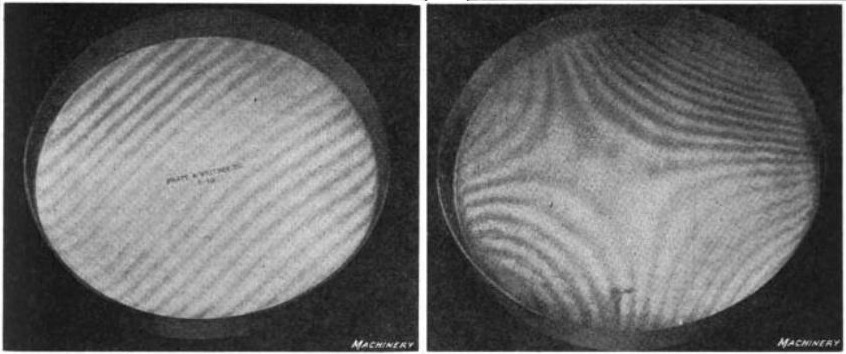
\includegraphics[width=0.62\linewidth]{images/book4/optical-flat-fringes.jpg}

{\small \omterm{prop:b2:two-wave-interference:film}{هدب تساوي السماكة} بين مستوٍ بصري وسطح فولاذي تحت الاختبار، في صورة فوتوغرافية لميكانيكي من نحو 1915: هدب مستقيمة فوق سطح مستوٍ، ومنحنية حيث تآكل --- وكل هدبة درجة قدرها نصف طول موجة.}
\end{omfigure}

\section{مسألة: مرآتا فرينل وغشاء زيت}

\begin{problem}[{مسألة نهاية الأسبوع --- مقياس تداخل من عام 1816 وقوس
قزح على بركة: طريقتان لشطر موجة واحدة، والترابطان
اللذان يحدّانهما معًا}]
\label{pb:b2:two-wave-interference:1}

\medskip
\noindent\textbf{الجزء الأول --- مرآتا فرينل.}
مرآتان مستويتان متلامستان على مستقيم تصنعان زاوية صغيرة جدًّا $\alpha =
\qty{5.0e-3}{rad}$؛ ومنبع شقّي $S$، موازٍ لذلك المستقيم، على $d =
\qty{20}{cm}$ منه، والشاشة على $D = \qty{1.5}{m}$ وراءه. و $\lambda =
\qty{589}{nm}$ (الصوديوم).
\begin{enumerate}
  \item بيّن أن المرآتين تعطيان صورتين تخيليتين $S_1$ و $S_2$ للمنبع
        $S$ على دائرة نصف قطرها $d$ مركزها مستقيم التماس،
        متباعدتين $a = 2\alpha d$؛ وأوجد قيمته.
  \item ولمَ تتداخل الموجتان الآتيتان من $S_1$ و $S_2$، بينما لا تتداخل
        موجتا مصباحين منفصلين؟
  \item وأوجد \omterm{prop:b2:two-wave-interference:young}{البعد الهدبي} على الشاشة (والبعد من المنبعين إلى
        الشاشة $\approx d + D$)؛ وعدد الهدب عبر
        المنطقة التي عرضها \qty{5}{mm} حيث تتراكب الحزمتان المنعكستان.
  \item \omterm{thm:b2:two-wave-interference:formula}{ورتبة التداخل} عند حرف تلك المنطقة؛ أهي دون
        الحدّ الذي يضعه طول ترابط المصباح (\qty{2}{cm})؟
  \item وشقّ المنبع عرضه \qty{20}{\micro m}: أوجد إزاحة الهدب
        الناتجة عن حرفيه (فكل نقطة منبع تُصوَّر في نقطتين
        تخيليتين؛ وينزاح نظام الهدب بمقدار $bD'/d$ مع $D' =
        d + D$)؛ أيُحفَظ التباين (قارن \omterm{prop:b2:two-wave-interference:young}{بالبعد الهدبي} $i$)؟
  \item ويُوسَّع الشقّ إلى \qty{0.1}{mm}: أوجد التباين، باستعمال
        $|\operatorname{sinc}(\pi ab/\lambda d)|$.
  \item وتعكس المرآتان $90\%$ و $80\%$ من الضوء: أوجد تباين
        الهدب.
  \item وتوضع صفيحة زجاجية سماكتها \qty{10}{\micro m} ($n = 1.5$)
        أمام إحدى المرآتين: أوجد إزاحة النقش، بالهدب؛ أيمكن
        تتبّعها بضوء الصوديوم؟ وبالضوء الأبيض؟
  \item واستبدل بالمصباح الصودي ضوءًا أبيض: صِف الشاشة؛
        وكم هدبة ملونة على كل جانب من المركز؟
\end{enumerate}

\medskip
\noindent\textbf{الجزء الثاني --- غشاء الزيت.}
غشاء زيت ($n = 1.45$) ينتشر على طريق مبلّل ($n_{\text{ماء}} = 1.33$)،
تضيئه سماء ملبّدة ويُنظر إليه قرب الورود الناظمي.
\begin{enumerate}[resume]
  \item الانعكاسان على الوجهين: أيّهما يعكس الإشارة؟ وأوجد \omterm{thm:b2:two-wave-interference:formula}{فرق
        المسير}؛ وشرط اللون المضيء.
  \item وسماكة أرقّ منطقة تبدو حمراء ($\lambda =
        \qty{650}{nm}$)؛ وخضراء (\qty{550}{nm})؛ وبنفسجية (\qty{420}{nm}).
  \item ومنطقة سماكتها \qty{600}{nm}: أيّ أطوال الموجة المرئية
        متعاضدة، وأيّها متلاشية؛ وما لونها؟
  \item ولمَ يُظهر الغشاء أشرطة من الألوان (وما الذي يتغير على امتداد
        الطريق)، ولمَ تتبع الأشرطة خطوط تساوي السماكة؟
  \item ويرقّ الغشاء بالتبخر: صِف تغير تتابع
        اللون عند نقطة معينة؛ وماذا يُرى حين $e \to 0$
        هنا --- أمضيء أم مظلم؟ وقارن ذلك بغشاء صابون في الهواء.
  \item وأعلى غشاء الصابون النازف يسودّ قبيل
        انفجاره: أوجد السماكة هناك (بضعة نانومترات) ولمَ السواد.
  \item ويُنظر إليه تحت الورود \qty{60}{\degree}: أوجد زاوية الانكسار في الزيت،
        وإزاحة أطوال الموجة المضيئة في السؤال 11.
  \item وبعد أي سماكة تخبو الألوان إلى رمادي
        منتظم، من أجل ضوء نهار طول ترابطه نحو \qty{1}{\micro m}؟
  \item وضوء السماء غير مستقطب ويصل من جهات
        كثيرة: فلمَ لا يُمحى النقش كما يمحو \omterm{prop:b2:two-wave-interference:spatial}{المنبع الممتد}
        هدب يونغ؟ (أي التوضيع على الغشاء.)
\end{enumerate}

\medskip
\noindent\textbf{الجزء الثالث --- الترابطان.}
\begin{enumerate}[resume]
  \item الترابط الزماني: أوجد أعظم رتبة مرئية من أجل مرآتي فرينل
        بضوء الصوديوم؛ ومع ليزر ($\ell_c = \qty{10}{m}$).
  \item \omterm{prop:b2:two-wave-interference:spatial}{والترابط المكاني}: أوجد أعظم عرض منبع من أجل المرآتين
        (من $ab/d < \lambda/4$) ومن أجل شقّي يونغ مع $a = \qty{1}{mm}$ على
        $L = \qty{40}{cm}$.
  \item وفسّر لمَ يحتمل الغشاء الرقيق منبعًا ممتدًّا بينما
        لا يحتمله \omterm{prop:b2:two-wave-interference:young}{شقّا يونغ}: ارسم شعاعي الغشاء من أجل نقطتي منبع
        مختلفتين وبيّن أنهما يظلان يلتقيان على الغشاء.
  \item وخط الصوديوم نفسه عرضه \qty{0.02}{nm}: فكم هدبة
        تستطيع المرآتان أن تُظهرا على الأكثر (استعمل $N \approx \lambda/\Delta\lambda$)؟
  \item ويستبدل طالب بالمصباح الصودي ثنائيًّا باعثًا للضوء أخضر ($\Delta\lambda =
        \qty{30}{nm}$): أوجد عدد الهدب المرئية مع المرآتين.
  \item ومع ليزر تمتد الهدب على منطقة التراكب كلها
        بتباين تامّ لكن الشاشة "مرقّطة": فلماذا؟
  \item وفي جدول واحد، من أجل المرآتين والغشاء: كيف تُشطر الموجة،
        وأين تُوضَّع الهدب، وما الذي يحدّ عددها،
        وماذا يفعل منبع أعرض.
\end{enumerate}
\end{problem}
